\section{RCRRTBall\-Ext\-Ext  Class Reference}
\label{classRCRRTBallExtExt}\index{RCRRTBallExtExt@{RCRRTBall\-Ext\-Ext}}
Dual tree version of {\bf RCRRTBall} {\rm (p.\,\pageref{classRCRRTBall})} with Ext\-Ext method. 


{\tt \#include $<$rcrrt.h$>$}

Inheritance diagram for RCRRTBall\-Ext\-Ext::\begin{figure}[H]
\begin{center}
\leavevmode
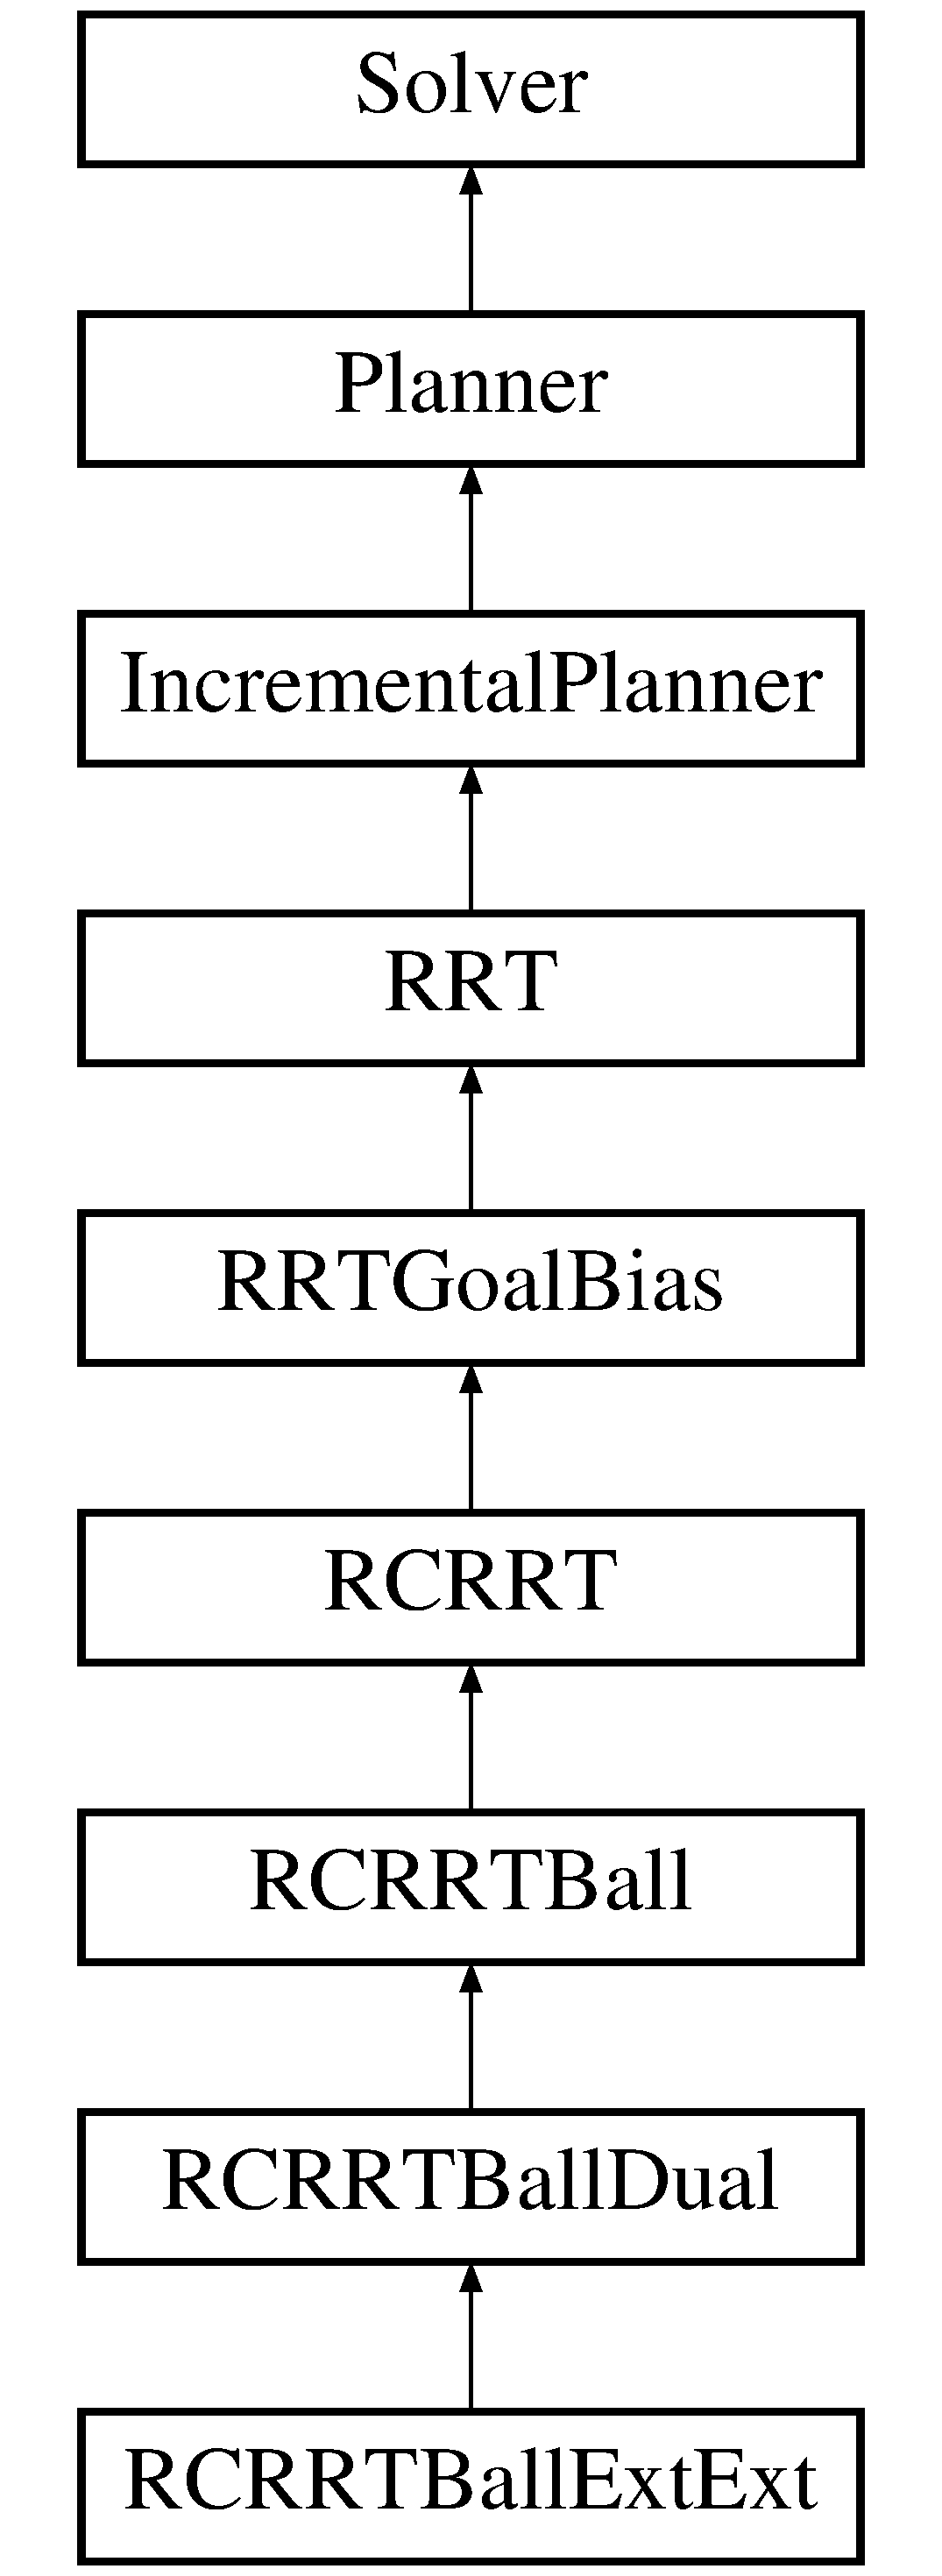
\includegraphics[height=9cm]{classRCRRTBallExtExt}
\end{center}
\end{figure}
\subsection*{Public Methods}
\begin{CompactItemize}
\item 
{\bf RCRRTBall\-Ext\-Ext} ({\bf Problem} $\ast$p)
\item 
virtual {\bf $\sim$RCRRTBall\-Ext\-Ext} ()
\item 
virtual bool {\bf Plan} ()
\begin{CompactList}\small\item\em Attempt to solve an Initial-Goal query by growing an {\bf RRT} {\rm (p.\,\pageref{classRRT})}.\item\end{CompactList}\end{CompactItemize}


\subsection{Detailed Description}
Dual tree version of {\bf RCRRTBall} {\rm (p.\,\pageref{classRCRRTBall})} with Ext\-Ext method.



\subsection{Constructor \& Destructor Documentation}
\index{RCRRTBallExtExt@{RCRRTBall\-Ext\-Ext}!RCRRTBallExtExt@{RCRRTBallExtExt}}
\index{RCRRTBallExtExt@{RCRRTBallExtExt}!RCRRTBallExtExt@{RCRRTBall\-Ext\-Ext}}
\subsubsection{\setlength{\rightskip}{0pt plus 5cm}RCRRTBall\-Ext\-Ext::RCRRTBall\-Ext\-Ext ({\bf Problem} $\ast$ {\em p})}\label{classRCRRTBallExtExt_a0}


\index{RCRRTBallExtExt@{RCRRTBall\-Ext\-Ext}!~RCRRTBallExtExt@{$\sim$RCRRTBallExtExt}}
\index{~RCRRTBallExtExt@{$\sim$RCRRTBallExtExt}!RCRRTBallExtExt@{RCRRTBall\-Ext\-Ext}}
\subsubsection{\setlength{\rightskip}{0pt plus 5cm}virtual RCRRTBall\-Ext\-Ext::$\sim$RCRRTBall\-Ext\-Ext ()\hspace{0.3cm}{\tt  [inline, virtual]}}\label{classRCRRTBallExtExt_a1}




\subsection{Member Function Documentation}
\index{RCRRTBallExtExt@{RCRRTBall\-Ext\-Ext}!Plan@{Plan}}
\index{Plan@{Plan}!RCRRTBallExtExt@{RCRRTBall\-Ext\-Ext}}
\subsubsection{\setlength{\rightskip}{0pt plus 5cm}bool RCRRTBall\-Ext\-Ext::Plan ()\hspace{0.3cm}{\tt  [virtual]}}\label{classRCRRTBallExtExt_a2}


Attempt to solve an Initial-Goal query by growing an {\bf RRT} {\rm (p.\,\pageref{classRRT})}.



Reimplemented from {\bf RCRRTBall\-Dual} {\rm (p.\,\pageref{classRCRRTBallDual_a2})}.

The documentation for this class was generated from the following files:\begin{CompactItemize}
\item 
{\bf rcrrt.h}\item 
{\bf rcrrt.C}\end{CompactItemize}
